% Provenance (never printed): see sources/outline_sources.md (Year 2: climate archives and proxies;
% foraminiferal and ice isotopes; Mg/Ca; pollen; speleothems; tree rings; dating the archives).
% Calibrations after Miller et al. (2020), Groeneveld et al. (2019) and Morley et al. (2024); ice
% cores after White (Geochemistry, ch. 9), Werner et al. (2018) and the EPICA Dome C file of Jouzel
% et al. (2007); age model after Svensson et al. (2008); deep-water context after Wharton et al.
% (2026); figures from figdata/bachelor-2/proxies.py (data/derived lr04, edc-temperature,
% co2-icecore); values of the exercises and problem computed in the Book 4 scratch calculator
% calc/ch24.py.
\chapter{Climate Archives and Proxies}\label{ch:b2:climate-proxies}

In a paper of 1955 a young geochemist reported the oxygen isotopes of the tiny shells of
foraminifera picked from cores of the ocean floor, and found in them fifteen glacial--interglacial cycles over the
last \num{600000} years. He read them mostly as temperature: he attributed only about a fifth of
the swings to the ice stored on land. Eighteen years later, Shackleton and Opdyke concluded the
opposite: the main effect was the storage of isotopically light water in the ice
sheets. The same shells, the same numbers, two readings. A shell of calcite records the
temperature of the water it grew in and the composition of that water, and the composition of
sea water depends on how much ice there is on land. This chapter is about such records, the
archives that keep them, the proxies read from them, how they are calibrated against thermometers
and how they are dated, and about the art of telling apart two signals carried by one shell.
% ledger: white13c9:paleo-history

\begin{recall}
\textbf{From the school volumes}: \omterm{def:b2:climate-proxies:proxy}{climate archive} and proxy, ice core, glacial period and
interglacial, the Last Glacial Maximum (about \num{23000} to \num{19000} years ago), pollen
analysis. \textbf{From the Year 1 volume}: radiometric dating, the radiocarbon age and its
calibration curve; calcareous ooze, made of coccoliths and the shells of foraminifera.
\textbf{From \cref{ch:b2:isotope-geochemistry}}: the \omterm{def:b2:isotope-geochemistry:standards}{isotope reference standards} \omterm{def:b2:isotope-geochemistry:standards}{VSMOW} and \omterm{def:b2:isotope-geochemistry:standards}{VPDB}
(\cref{def:b2:isotope-geochemistry:standards}) and the \omterm{prop:b2:isotope-geochemistry:mwl}{meteoric water line}, $\delta\mathrm{D}
\approx 8\,\delta^{18}\mathrm{O} + 10$ (\cref{prop:b2:isotope-geochemistry:mwl}). \textbf{From the
chemistry books}: the $\delta$ value and the fractionation factor. \textbf{From the mathematics
books}: the least-squares line.
\end{recall}
% ledger: ipcc:lgm-cooling, kc98:mwl, kc98:standards

\section{Archives and proxies}\label{sec:b2:climate-proxies:archives}

Instruments have measured the climate only recently. Everything earlier is read from materials
that grew or settled layer by layer while the climate acted on them: snow turning to ice on the
polar ice sheets, shells raining onto the ocean floor, the rings of trees, corals, the deposits of
caves, the mud of lakes. The school volumes called them archives and the quantities measured in
them proxies; we now need sharper words.

\begin{definition}[Climate archive; climate proxy]\label{def:b2:climate-proxies:proxy}
A \emph{climate archive}\index{climate archive} is a natural material that accumulates
progressively, layer upon layer or ring upon ring, and preserves physical, chemical or biological
characteristics of the environment in which each part formed. A \emph{climate
proxy}\index{climate proxy} is a quantity measured in an archive that depends on a climate
variable, such as a temperature, an amount of rain or a volume of ice, through a relation that can
be calibrated, and so stands in for a measurement of that variable that was never made.
\end{definition}
% ledger: ncei:proxy, ncei:paleocean

Three properties decide what an archive can tell: its resolution (the time span covered by one
sample), its reach (how far back it goes) and how it is dated. An archive with annual layers can be
read year by year and dated by counting; the others need radiometric ages or comparison with a
dated record. The table below compares the archives of this chapter.

\begin{center}
\small
\begin{tabular}{>{\raggedright\arraybackslash}p{0.17\linewidth}>{\raggedright\arraybackslash}p{0.27\linewidth}>{\raggedright\arraybackslash}p{0.21\linewidth}>{\raggedright\arraybackslash}p{0.24\linewidth}}
\hline
archive & proxies in this chapter & annual layers & dating \\
\hline
deep-sea sediment & $\delta^{18}$O and Mg/Ca of foraminifera & no & radiocarbon, comparison with
dated records \\
polar ice & $\delta$D and $\delta^{18}$O of the ice, air in bubbles & in the upper part of thick
cores & counting layers, dated volcanic layers \\
tree rings & ring width, wood density, isotopes & yes & counting and \omterm{def:b2:climate-proxies:dendro}{cross-dating} rings \\
\omterm{def:b2:climate-proxies:archives}{speleothems} & $\delta^{18}$O & in some & radiometric dating \\
lake sediments & \omterm{def:b2:climate-proxies:archives}{varves}, pollen & where varved & counting \omterm{def:b2:climate-proxies:archives}{varves} \\
\hline
\end{tabular}
\end{center}
% ledger: ncei:proxy, ncei:paleocean, ncei:tree-ring, ncei:speleothem, mccarthy23:varves, svensson08:gicc05, noaa:gisp2-layers, bebchuk26:crossdating

A proxy is never a pure measure of one variable. The width of a tree ring depends on the warmth of
the summer and on the rain; the $\delta^{18}$O of a shell on the temperature of the water and on
its isotopic composition. The work of the palaeoclimatologist is to find a proxy whose dependence
on the variable sought is strong and known, to measure the other influences independently, and to
date the sample.

\section{Oxygen isotopes in carbonate shells}\label{sec:b2:climate-proxies:oxygen}

Foraminifera are single-celled protists, many of which build a shell of calcite; the planktonic
species float in the surface waters, the benthic ones live on or in the sediment of the sea
floor. Their shells accumulate in the calcareous oozes of the Year 1 volume, and the
$\delta^{18}$O of the calcite can be measured on a few shells picked from each centimetre of a
core.
% ledger: ucmp:forams, ncei:paleocean

\begin{history}[Two readings of one record]
Urey calculated in 1947 how the fractionation of oxygen between calcite and water depends on
temperature, and proposed that carbonates could record the temperature at which they formed. Cesare
Emiliani, then his student, measured $\delta^{18}$O in foraminifera from piston cores of the
world's oceans and published in 1955 a record with 15 glacial--interglacial cycles over
\num{600000} years, attributing about \qty{20}{\percent} of the variation to the volume of ice.
In 1973 Shackleton and Opdyke concluded that the storage of isotopically light water in the
ice sheets was the main effect. The vital effects, the departures of a species from equilibrium,
and the exchange of oxygen with pore water after burial are usually not very important for the
shells of the last few million years; the isotopic composition of the water is.
\end{history}
% ledger: white13c9:paleo-history

\subsection*{Temperature}

Calcite that grows in equilibrium with water is richer in \textsuperscript{18}O than the water,
and the colder the water, the larger the enrichment, as Urey's calculation showed. Several
empirical calibrations relate
temperature to the difference between the $\delta^{18}$O of the calcite, on the \omterm{def:b2:isotope-geochemistry:standards}{VPDB} scale, and
that of the water, on the \omterm{def:b2:isotope-geochemistry:standards}{VSMOW} scale. For the deep sea, one simplified form is used for benthic
shells.

\begin{proposition}[A benthic calibration]\label{prop:b2:climate-proxies:benthic}
For benthic foraminifera at deep-sea temperatures (below about \qty{13}{\celsius}),
\[
  T = 16.1 - 4.76\,\bigl[\delta^{18}\mathrm{O}_{\mathrm{b}} - (\delta^{18}\mathrm{O}_{\mathrm{sw}} -
  0.27)\bigr],
\]
with $T$ in \unit{\celsius}, $\delta^{18}\mathrm{O}_{\mathrm{b}}$ the value of the shell (per mil,
\omterm{def:b2:isotope-geochemistry:standards}{VPDB}) and $\delta^{18}\mathrm{O}_{\mathrm{sw}}$ that of the sea water (per mil, \omterm{def:b2:isotope-geochemistry:standards}{VSMOW}); the term
0.27 converts the water to the scale of the calcite. A cooling of \qty{1}{\celsius} at constant
water composition raises $\delta^{18}\mathrm{O}_{\mathrm{b}}$ by $1/4.76 = 0.21$ per mil.
\end{proposition}
\admitted
% ledger: miller20:paleotemp, groeneveld19:anand

The fuller equation from which it is simplified carries a small quadratic term,
$T = 16.1 - 4.64x + 0.09x^2$ with $x$ the difference of the two $\delta$ values; planktonic shells
have their own calibrations, of the same form, such as $T = 14.9 - 4.8\,[\delta^{18}\mathrm{O} -
(\delta^{18}\mathrm{O}_{\mathrm{sw}} - 0.27)]$. All share one difficulty: the shell gives one
number, $\delta^{18}\mathrm{O}_{\mathrm{b}}$, and the equation has two unknowns, $T$ and
$\delta^{18}\mathrm{O}_{\mathrm{sw}}$. A second, independent proxy is needed to separate them.
% ledger: miller20:paleotemp, groeneveld19:anand

\subsection*{The ice-volume effect}

Water evaporating from the sea carries less \textsuperscript{18}O than the sea; as the vapour
travels poleward and rains or snows out, it is depleted further, and the snow that builds the ice
sheets is among the lightest water on the planet: Greenland ice has a $\delta^{18}$O of $-30$ to $-35$
per mil, Antarctic ice as low as $-50$. When ice sheets grow, the light isotope is locked on land
and the ocean left behind becomes heavier.
% ledger: nasaeo:o18, white:d18o

\begin{definition}[Ice-volume effect]\label{def:b2:climate-proxies:ice-volume}
The \emph{ice-volume effect}\index{ice-volume effect} is the change of the oxygen-isotope
composition of the whole ocean caused by the growth or decay of the continental ice sheets, which
store water depleted in \textsuperscript{18}O; it shifts the $\delta^{18}$O of every carbonate
formed in the sea by the same amount, whatever the temperature.
\end{definition}
% ledger: nasaeo:o18, white13c9:ice-volume, miller20:paleotemp

\begin{omfigure}
\centering
\begin{tikzpicture}[font=\scriptsize, >=Stealth]
\foreach \col/\title in {0/{a\enspace today}, 7.0/{b\enspace a glacial maximum}} {
  \begin{scope}[shift={(\col,0)}]
  \node[anchor=south west] at (0,3.3) {\textbf{\title}};
  \fill[brown!30] (3.6,0) -- (6.4,0) -- (6.4,1.6) -- (3.6,1.2) -- cycle;
  \end{scope}
}
% today: full ocean, small ice sheet
\fill[ocBlue!25] (0,0) rectangle (3.6,1.2);
\node[align=center] at (1.75,0.55) {ocean\\$\delta^{18}\mathrm{O} = 0$};
\fill[white, draw=black!50] (5.2,1.43) .. controls (5.6,1.95) and (6.2,1.95) .. (6.4,1.6) -- cycle;
\node at (5.0,0.65) {ice, $-40$};
\draw[black!50] (5.0,0.85) -- (5.7,1.55);
\draw[->, thick, ocBlue] (1.6,1.35) .. controls (2.4,2.9) and (4.6,2.9) .. (5.6,2.05);
\node at (3.4,3.0) {vapour, light};
% glacial: lower sea, big ice sheet
\begin{scope}[shift={(7.0,0)}]
\fill[ocBlue!35] (0,0) rectangle (3.6,0.85);
\draw[densely dashed] (0,1.2) -- (3.6,1.2);
\node[anchor=south west, align=left] at (0.05,1.2) {today's\\sea level};
\draw[<->] (3.35,0.85) -- (3.35,1.2);
\node[anchor=east] at (3.3,1.02) {\qty{130}{m}};
\node[align=center] at (1.6,0.42) {ocean, $\delta^{18}\mathrm{O} = +1.46$};
\fill[white, draw=black!50] (3.6,1.2) .. controls (4.0,2.6) and (6.0,2.7) .. (6.4,1.6) -- cycle;
\node at (5.1,1.85) {ice, $-40$};
\draw[->, thick, ocBlue] (2.15,0.9) .. controls (2.3,2.6) and (3.3,3.0) .. (4.3,2.6);
\end{scope}
\end{tikzpicture}
\par\smallskip{\small The \omterm{def:b2:climate-proxies:ice-volume}{ice-volume effect} (schematic, not to scale): the vapour that feeds the ice
sheets is depleted in \textsuperscript{18}O, so storing \qty{130}{m} of sea level as ice of
$\delta^{18}\mathrm{O} = -40$ per mil leaves the ocean \num{1.46} per mil heavier
(\cref{prop:b2:climate-proxies:mass-balance}). Values in per mil, \omterm{def:b2:isotope-geochemistry:standards}{VSMOW}.}
\end{omfigure}
% ledger: nasaeo:o18, miller20:ice-cal, ipcc:lgm-sea

How large is the shift? A mass balance answers it, if the volume of the ice and its mean isotopic
composition are known.

\begin{proposition}[Ice-volume effect by mass balance]\label{prop:b2:climate-proxies:mass-balance}
Let the present ocean have mean depth $H$ and a $\delta^{18}$O of 0 (\omterm{def:b2:isotope-geochemistry:standards}{VSMOW}). If a layer of sea
water of thickness $h$ is removed and stored on land as ice of mean composition
$\delta_{\mathrm{ice}}$, the area of the ocean being held fixed, the remaining ocean has
\[
  \Delta\delta^{18}\mathrm{O}_{\mathrm{sw}} = \frac{-h\,\delta_{\mathrm{ice}}}{H - h}.
\]
For small $h$ the shift grows nearly linearly, by $-\delta_{\mathrm{ice}}/H$ per metre of sea level.
\end{proposition}

\begin{proof}
For a minor isotope, $\delta$ values combine like concentrations: the $\delta$ of a mixture is
the mean of the $\delta$ values of its parts weighted by their amounts of oxygen, and all the
parts here are water. Per unit of ocean area, the water of the present ocean, a column $H$ at
$\delta = 0$, is shared between the ice, $h$ at $\delta_{\mathrm{ice}}$, and the remaining ocean,
$H - h$ at $\Delta\delta^{18}\mathrm{O}_{\mathrm{sw}}$:
$H \times 0 = h\,\delta_{\mathrm{ice}} + (H - h)\,\Delta\delta^{18}\mathrm{O}_{\mathrm{sw}}$, which
gives the formula. For $h \ll H$, $H - h \approx H$.
\end{proof}
% ledger: white13c9:ice-mass, charette:ocean-volume

\begin{example}[The last glacial ocean]\label{ex:b2:climate-proxies:lgm}
At the Last Glacial Maximum sea level stood 125 to \qty{134}{m} below today's; take \qty{130}{m},
with $H = \qty{3682.2}{m}$, and ice at $-40$ per mil, the value inferred for the great North
American ice sheet. Then
$\Delta\delta^{18}\mathrm{O}_{\mathrm{sw}} = 130 \times 40/(3682.2 - 130) = 5200/3552.2 = 1.46$
per mil, about $40/3682.2 = 0.0109$ per mil per metre of sea level. Comparisons of sea-level curves
from dated terraces and coral reefs give \num{0.011} per mil per metre, in agreement; a scaling of
\num{0.13} per mil per \qty{10}{m}, used in some reconstructions, corresponds to ice at about
$-50$ per mil. A direct measurement of the change, from the $\delta^{18}$O of the water still held
in the pores of glacial sediment, gives $1.0 \pm 0.1$ per mil.
\end{example}
% ledger: ipcc:lgm-sea, charette:ocean-volume, miller20:ice-cal, white13c9:ice-volume, wharton26:deep

The figure below shows how strongly the answer depends on the composition assumed for the ice.
The difference between \num{1.0} and \num{1.5} per mil is not small: at \num{0.21} per mil per degree,
it is worth more than two degrees of deep-ocean temperature. The relation is also not quite
linear: the ocean that remains shrinks as the ice grows, and the mean $\delta^{18}$O of the ice
itself changes as ice sheets of different composition grow and decay. Reconstructions of sea level
from $\delta^{18}$O therefore often use a linear relation calibrated on the pore-water value, while
recognising that the true relation should be nonlinear.
% ledger: wharton26:deep, rohling21:linear, miller20:paleotemp

\begin{omfigure}
\centering
% figdata/bachelor-2/proxies.py part icevol
\begin{tikzpicture}
\begin{axis}[width=0.86\linewidth, height=6.0cm, xmin=0, xmax=150, ymin=0, ymax=2.2,
  xlabel={sea water stored as ice, $h$ (\unit{m} of sea level)},
  ylabel={$\Delta\delta^{18}\mathrm{O}_{\mathrm{sw}}$ (per mil)},
  tick label style={font=\scriptsize}, label style={font=\small}, xtick={0,25,...,150},
  legend style={font=\scriptsize, at={(0.5,1.02)}, anchor=south, draw=none, legend columns=4,
  /tikz/every even column/.append style={column sep=6pt}}, legend cell align=left]
\fill[black!10] (axis cs:125,0) rectangle (axis cs:134,2.2);
\addplot[ocBlue, thick] table[x=h_m, y=d30] {figdata/out/bachelor-2-proxies-icevol.dat};
\addlegendentry{ice at $-30$}
\addplot[black, thick] table[x=h_m, y=d40] {figdata/out/bachelor-2-proxies-icevol.dat};
\addlegendentry{ice at $-40$}
\addplot[ocRed, thick] table[x=h_m, y=d50] {figdata/out/bachelor-2-proxies-icevol.dat};
\addlegendentry{ice at $-50$}
\addplot[only marks, mark=square*, mark size=1.8pt, omDef, error bars/.cd, y dir=both,
  y explicit] coordinates {(130,1.0) +- (0,0.1)};
\addlegendentry{pore water}
\addplot[black!60, densely dashed, domain=0:150, samples=2, forget plot] {1.69};
\node[font=\scriptsize, anchor=south west] at (axis cs:3,1.69) {whole LR04 change, 1.69};
\node[font=\scriptsize, anchor=north, align=center] at (axis cs:112,0.45) {last glacial\\maximum
$\rightarrow$};
\end{axis}
\end{tikzpicture}
\par\smallskip{\small The \omterm{def:b2:climate-proxies:ice-volume}{ice-volume effect} from the mass balance of
\cref{prop:b2:climate-proxies:mass-balance}, for three compositions of the ice (per mil, \omterm{def:b2:isotope-geochemistry:standards}{VSMOW});
grey band: the sea-level fall of the Last Glacial Maximum, 125 to \qty{134}{m}; square: the change
measured in sediment pore waters, $1.0 \pm 0.1$ per mil, placed at \qty{130}{m}; dashed: the
change of the benthic stack between today and the Last Glacial Maximum.}
\end{omfigure}
% ledger: ipcc:lgm-sea, wharton26:deep, data:b4-proxies, miller20:ice-cal

\subsection*{The benthic stack}

Records of benthic $\delta^{18}$O from many cores, aligned and averaged, form a stack whose noise
is lower than that of any single core. The LR04 stack combines 57 records from sites spread over the
world ocean and spans 5.3 million years. Between today, \num{3.23} per mil, and the mean of
\num{19} to \qty{23}{ka}, \num{4.92} per mil, it changes by \num{1.69} per mil, more than any
plausible \omterm{def:b2:climate-proxies:ice-volume}{ice-volume effect}. As Shackleton and Opdyke concluded, most of the change is the ice;
but a few tenths of a per mil remain for the deep water to have cooled. The problem of this chapter measures that residual.
% ledger: lr04:stack, data:b4-proxies, white13c9:paleo-history, wharton26:deep

\begin{omfigure}
\centering
% figdata/bachelor-2/proxies.py parts lr04, edc, co2
\begin{tikzpicture}
\begin{groupplot}[group style={group size=1 by 3, vertical sep=0.35cm, xlabels at=edge bottom,
  xticklabels at=edge bottom},
  width=0.96\linewidth, height=3.7cm, xmin=0, xmax=800, xtick={0,100,...,800},
  tick label style={font=\scriptsize}, label style={font=\small}]
\nextgroupplot[ylabel={$\delta^{18}\mathrm{O}_{\mathrm{b}}$}, y dir=reverse, ymin=2.45, ymax=5.2,
  ytick={3.5,4.5}]
\addplot[omDef, thin] table[x=age_ka, y=d18O] {figdata/out/bachelor-2-proxies-lr04.dat};
\node[font=\scriptsize, anchor=north east] at (rel axis cs:0.99,0.97) {a\enspace LR04 stack (per
mil, VPDB; axis reversed)};
\nextgroupplot[ylabel={$\Delta T$ (\unit{\celsius})}, ymin=-12, ymax=7, ytick={-10,-5,0,5}]
\addplot[ocBlue, thin] table[x=age_ka, y=dT] {figdata/out/bachelor-2-proxies-edc.dat};
\node[font=\scriptsize, anchor=north east] at (rel axis cs:0.99,0.97) {b\enspace EPICA Dome C
temperature anomaly};
\nextgroupplot[ylabel={CO$_2$ (\unit{ppm})}, ymin=160, ymax=330, ytick={200,250,300},
  xlabel={age (thousands of years before 1950)}]
\addplot[ocRed, thin] table[x=age_ka, y=co2] {figdata/out/bachelor-2-proxies-co2.dat};
\node[font=\scriptsize, anchor=north east] at (rel axis cs:0.99,0.97) {c\enspace CO$_2$ of
Antarctic ice-core air};
\end{groupplot}
\end{tikzpicture}
\par\smallskip{\small The last \num{800000} years in three archives: (a) the LR04 benthic
$\delta^{18}$O stack, plotted with its axis reversed so that glacial times point down; (b) the
temperature anomaly at EPICA Dome C, relative to the mean of the last thousand years, derived from
the $\delta$D of the ice; (c) the CO$_2$ of the air trapped in Antarctic ice, to 1950. Data: NOAA
NCEI Paleoclimatology (Lisiecki and Raymo 2005; Jouzel et al.\ 2007; Bereiter et al.\ 2015), as
fetched on 22 October 2026.}
\end{omfigure}
% ledger: data:lr04, data:edc-jouzel, data:co2-bereiter, jouzel07:edc-corr, data:b4-proxies

\section{Ice cores}\label{sec:b2:climate-proxies:ice}

The snow that falls on an ice sheet keeps the isotopic composition it had when it fell, and the
colder the place and the time, the lighter it is. In Antarctica the annual mean air temperature and
the $\delta^{18}$O of the snow follow a strong linear relation from one site to another, with a
slope of about \num{0.8} per mil per degree, as the Rayleigh distillation of the vapour on its way
inland predicts. Hydrogen is used as much as oxygen: on the \omterm{prop:b2:isotope-geochemistry:mwl}{meteoric water line}, $\delta$D varies about eight times as fast as $\delta^{18}$O, and
the $\delta$D record of Antarctic ice was chosen for its greater sensitivity to temperature.
% ledger: werner18:slopes, white13c9:icecore, kc98:mwl

A slope measured across space is not necessarily a slope in time. In Greenland, where the ice
temperature itself has been reconstructed by other methods, the change of $\delta^{18}$O per degree
over time turns out to be 0.3 to \num{0.6} per mil, against a present spatial slope of about
\num{0.7}: the seasons of snowfall, the sources of the moisture and its paths changed with the
climate. The early Antarctic temperatures were computed with a spatial relation measured in
the snow; more recent ones use general circulation models that simulate the water isotopes.
% ledger: werner18:slopes, white13c9:icecore

The core of EPICA Dome C, drilled through \qty{3260}{m} of ice, reaches \num{800000} years. Its
$\delta$D was measured on samples \qty{55}{cm} long, with an accuracy of \num{0.5} per mil, and
converted to a temperature anomaly relative to the average of the last thousand years, after
correcting for the changing composition of the sea water that fed the snow and for the changing
elevation of the ice sheet. Between glacial and interglacial times the temperature varied by about
\qty{15}{\celsius}. Between the last two thousand years and the Last Glacial Maximum (\num{19} to
\qty{23}{ka}), the mean $\delta$D falls from $-396.6$ to $-441.7$ per mil and the anomaly from
$-0.09$ to \qty{-9.39}{\celsius}.
% ledger: white13c9:icecore, jouzel07:edc-corr, jouzel07:edc, data:b4-proxies

Ice also keeps air. The firn, the packed snow of the top tens of metres, is open to the
atmosphere until its pores close off at the transition to ice, 50 to \qty{120}{m} down; the air
in a bubble is therefore younger than the ice around it. Measured in the bubbles, the CO$_2$ of the
air was \qty{189.7}{ppm} on average between \num{19} and \qty{23}{ka}, and \qty{279.4}{ppm} over
the two thousand years before industry. The panels (b) and (c) of the figure above rise and fall
together over the last \num{800000} years.
% ledger: firn:close-off, data:b4-proxies-co2, data:co2-bereiter

Greenland cores reach only about \num{120000} years, but the snow accumulates faster there and
the record is finer; it shows the abrupt warmings of the last glacial period known as the
Dansgaard--Oeschger events. Near the top of a thick core, the seasons themselves can be seen.
% ledger: white13c9:icecore

\begin{omfigure}
\centering
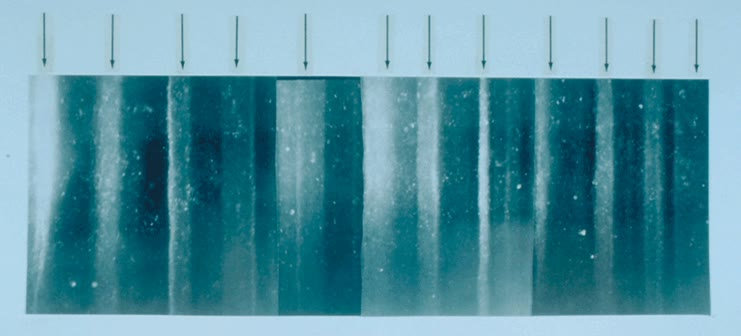
\includegraphics[width=0.72\linewidth]{images/book4/b2-24-gisp2-layers.jpg}
\par\smallskip{\small A section of the GISP2 ice core of central Greenland from \qty{1855}{m}
depth, lit from below, with alternating summer and winter layers (the arrows are those of the
original slide). During the dry northern summer, dust from Arctic Canada and coastal Greenland is
carried by the wind onto the ice sheet.
(Anthony Gow, U.S.\ Army Corps of Engineers CRREL, NOAA Paleoclimatology slide set, public domain,
via Wikimedia Commons.)}
\end{omfigure}
% ledger: photo:b2-24-gisp2, noaa:gisp2-layers

\begin{inthelab}[Cutting an ice core]
\begin{minipage}[t]{0.54\linewidth}\vspace{0pt}
At a national ice-core facility, the cores are kept in tubes, one metre of core per tube, in an
archive freezer at \qty{-36}{\celsius}; the scientists work in an examination room at
\qty{-24}{\celsius}. When a new core arrives, a core processing line forms: scientists and
staff measure, catalogue and cut each section, at typically 30 to \qty{35}{m} a day, so that a
core \qty{1000}{m} long takes six to eight weeks. One researcher shaves the core smooth with a
planer and measures its electrical conductivity, a key to defining and dating the layers; another
saws the pieces whose trapped air will be analysed for carbon dioxide and methane; the samples are
then shipped to the laboratories that measure them. At EPICA Dome C, each sample of the $\delta$D
profile was \qty{55}{cm} of ice.
\end{minipage}\hfill
\begin{minipage}[t]{0.42\linewidth}\vspace{0pt}
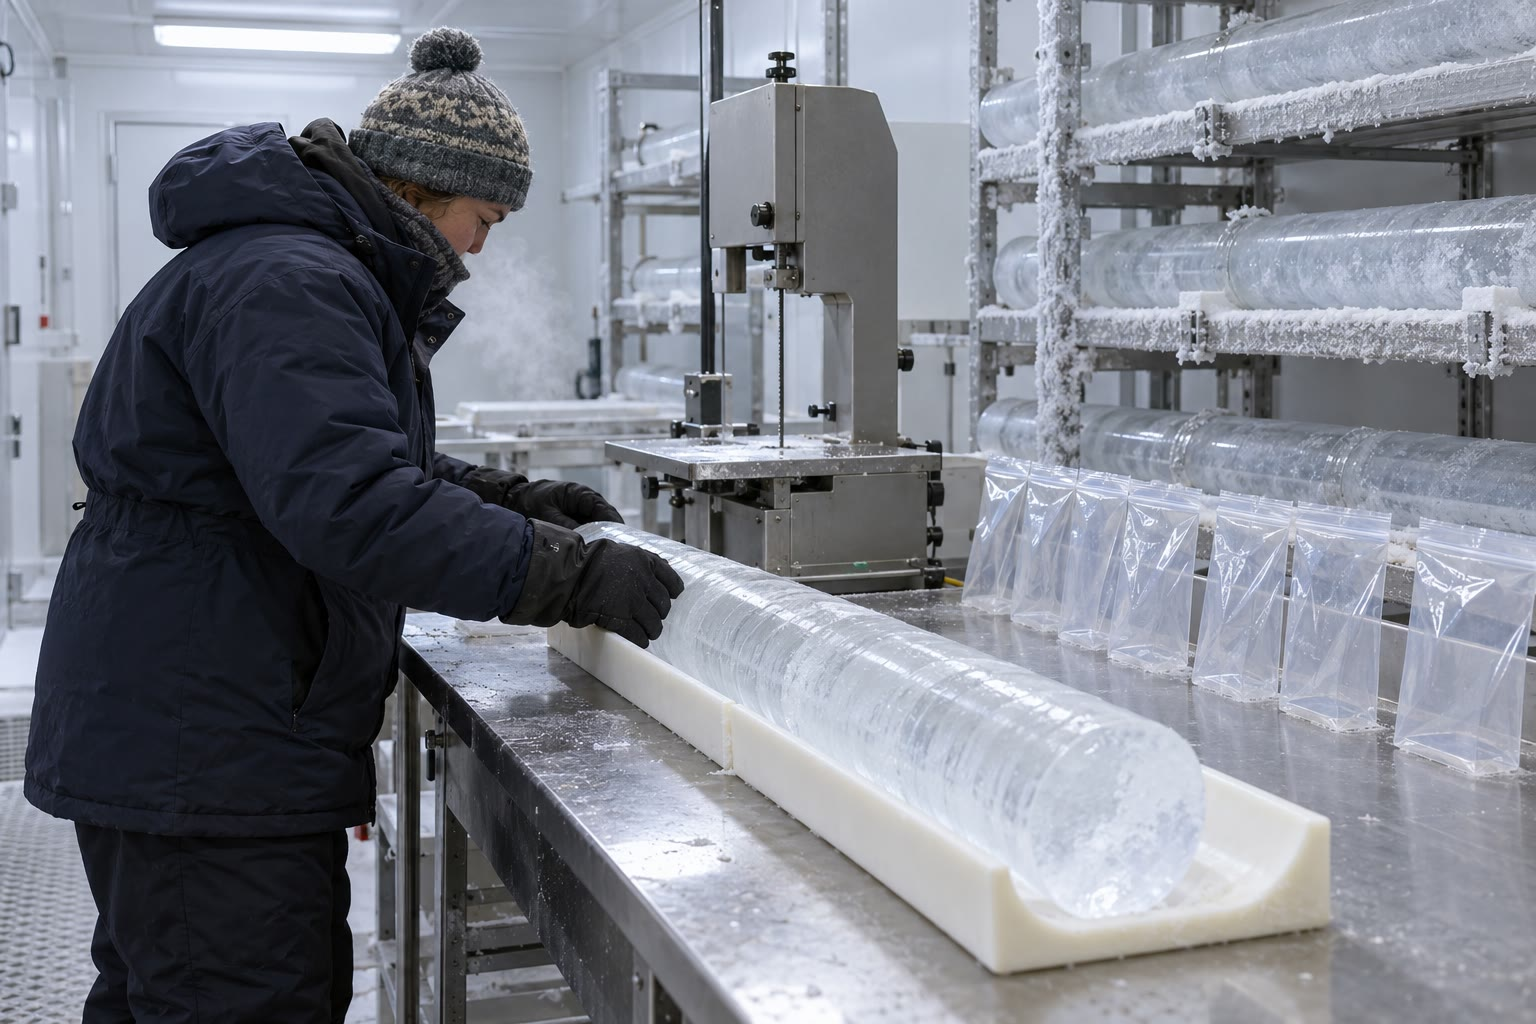
\includegraphics[width=\linewidth]{images/book4/ai/b2-24-cold-lab.jpg}

{\scriptsize A length of ice core on the bench of a cold laboratory, beside a band saw and sample
bags (AI-generated illustration).}
\end{minipage}
\end{inthelab}
% ledger: nsficf:cpl, jouzel07:edc-corr

\section{Other proxies, other archives}\label{sec:b2:climate-proxies:others}

\subsection*{The magnesium of shells}

The calcite of foraminifera takes up a little magnesium in place of calcium, and more of it when
the water is warmer. The ratio does not depend on the isotopic composition of the water, so it
gives the temperature that the $\delta^{18}$O equation needs.

\begin{definition}[Mg/Ca ratio (proxy)]\label{def:b2:climate-proxies:mgca}
The \emph{Mg/Ca ratio (proxy)}\index{Mg/Ca ratio (proxy)} is the ratio of magnesium to calcium in
the calcite of foraminiferal shells, in \unit{mmol/mol}, used as a measure of the temperature of
the water in which the shell grew through an exponential calibration
\[
  \text{Mg/Ca} = B\,\mathrm{e}^{A T},
\]
with $A$ close to \qty{0.09}{\per\celsius} for planktonic species and $B$ specific to the species.
\end{definition}
% ledger: groeneveld19:anand, morley24:mgca, miller20:paleotemp

With $A = 0.09$ the ratio grows by $\mathrm{e}^{0.09} - 1 = \qty{9.4}{\percent}$ per degree,
whatever the temperature. For one planktonic species of cold waters, the calibration predicted from
temperature alone is $\text{Mg/Ca} = 0.4\,\mathrm{e}^{0.09T}$; a fit to 235 shells from plankton
tows and the tops of North Atlantic cores gives $0.372\,\mathrm{e}^{0.0936T}$, with $r^2 = 0.90$.
At low temperatures the measured ratios depart from the curve, and the departure is attributed to
the concentration of carbonate ion in the sea water: a proxy rarely depends on one variable only.
Benthic species are less sensitive, about \qty{0.1}{mmol/mol} per degree for low-magnesium
species living in the sediment.
% ledger: morley24:mgca, wharton26:deep

\begin{omfigure}
\centering
% figdata/bachelor-2/proxies.py part calib
\begin{tikzpicture}
\begin{groupplot}[group style={group size=2 by 1, horizontal sep=1.7cm},
  tick label style={font=\scriptsize}, label style={font=\small}, height=5.2cm,
  width=0.48\linewidth]
\nextgroupplot[xmin=-2, xmax=14, ymin=0, ymax=3.8, xlabel={$T$ (\unit{\celsius})},
  ylabel={$\delta^{18}\mathrm{O}_{\mathrm{b}} - \delta^{18}\mathrm{O}_{\mathrm{sw}}$ (per mil)},
  xtick={0,4,...,12}, title={a\enspace benthic $\delta^{18}$O}, title style={font=\scriptsize}]
\addplot[black, thick] table[x=T, y=dd_benthic] {figdata/out/bachelor-2-proxies-calib.dat};
\nextgroupplot[xmin=0, xmax=30, ymin=0, ymax=6.5, xlabel={$T$ (\unit{\celsius})},
  ylabel={Mg/Ca (\unit{mmol/mol})}, xtick={0,5,...,30}, title={b\enspace planktonic Mg/Ca},
  title style={font=\scriptsize},
  legend style={font=\scriptsize, at={(0.03,0.97)}, anchor=north west, draw=none},
  legend cell align=left]
\addplot[ocRed, thick] table[x=T, y=mgca_pred] {figdata/out/bachelor-2-proxies-calib.dat};
\addlegendentry{$0.4\,\mathrm{e}^{0.09T}$}
\addplot[ocBlue, thick, densely dashed] table[x=T, y=mgca_fit]
  {figdata/out/bachelor-2-proxies-calib.dat};
\addlegendentry{$0.372\,\mathrm{e}^{0.0936T}$}
\end{groupplot}
\end{tikzpicture}
\par\smallskip{\small Two calibrations. (a) The benthic calibration of
\cref{prop:b2:climate-proxies:benthic}: the calcite is heavier than the water (on their own
scales) by \num{0.21} per mil more for each degree of cooling. (b) The Mg/Ca of a planktonic
species, as predicted from temperature alone and as fitted to 235 shells.}
\end{omfigure}
% ledger: miller20:paleotemp, morley24:mgca

Measured on the same shells, Mg/Ca and $\delta^{18}$O give two equations for two unknowns: Mg/Ca
gives $T$, and \cref{prop:b2:climate-proxies:benthic} then gives
$\delta^{18}\mathrm{O}_{\mathrm{sw}}$, the ice-volume signal. Applied to benthic shells of the deep
North-West Atlantic, the method finds the water of the Last Glacial Maximum only about
\qty{2}{\celsius} colder than today's ($-1.78 \pm \qty{0.56}{\celsius}$), while estimates from
pore waters put both deep water masses near freezing in the glacial ocean, $-1.1$ and
\qty{-1.9}{\celsius}, where today they are at 2 to \qty{4}{\celsius} and 0 to \qty{1}{\celsius}.
% ledger: miller20:paleotemp, wharton26:deep

\subsection*{Tree rings}

\begin{definition}[Dendroclimatology; cross-dating]\label{def:b2:climate-proxies:dendro}
\emph{Dendroclimatology}\index{dendroclimatology} is the reconstruction of past climate from the
annual growth rings of trees: their width, the density of their wood and their isotopic
composition. \emph{Cross-dating}\index{cross-dating} is the matching of the pattern of wide and
narrow rings between trees, which assigns to every ring its absolute calendar year and reveals
rings that are locally absent in a single tree.
\end{definition}
% ledger: bebchuk26:crossdating, bebchuk26:absent-rings, ncei:tree-ring, ncei:proxy

A ring is wider when conditions favour growth. \omterm{def:b2:climate-proxies:dendro}{Cross-dating} is reliable at climatically extreme sites, where one
climate factor limits the growth of all the trees, so that they share the same pattern; it may
fail where no single factor dominates, and where many rings are locally absent.
Overlapping the patterns of living trees, old timbers and buried wood extends a chronology back
year by year; a recent study dated a chronology of 100 subfossil yews of eastern England to the
456 years from 2668 to 2213 BCE, using the $\delta^{18}$O of more than \num{1500} of their rings
against an absolutely dated oak chronology. The International Tree-Ring Data Bank holds the ring
widths, densities, isotopes and chronologies of more than \num{5000} sites on six continents.
% ledger: ncei:proxy, bebchuk26:crossdating, bebchuk26:absent-rings, ncei:tree-ring

\subsection*{Caves and lakes}

\begin{definition}[Speleothem; varve]\label{def:b2:climate-proxies:archives}
A \emph{speleothem}\index{speleothem} is a mineral deposit formed from groundwater within a
cave: stalagmites, stalactites and other forms. A \emph{varve}\index{varve} is
the deposit of one year in a lake or sea floor sediment, usually a pair of laminae of contrasting
composition, one laid down in summer and one in the rest of the year.
\end{definition}
% ledger: ncei:speleothem, mccarthy23:varves

\omterm{def:b2:climate-proxies:archives}{Speleothems} grow layer by layer from the groundwater that reaches a cave; the thickness of
their layers and their isotopic records give past climate conditions. Some are annually banded,
and some contain compounds that can be dated radiometrically. The time scale of the Greenland cores agrees with that of
the \omterm{def:b2:climate-proxies:archives}{speleothems} of Hulu Cave to within 800 years over the last \num{60000} years: two
archives, dated by different methods, check each other.
% ledger: ncei:speleothem, svensson08:gicc05

\begin{omfigure}
\centering
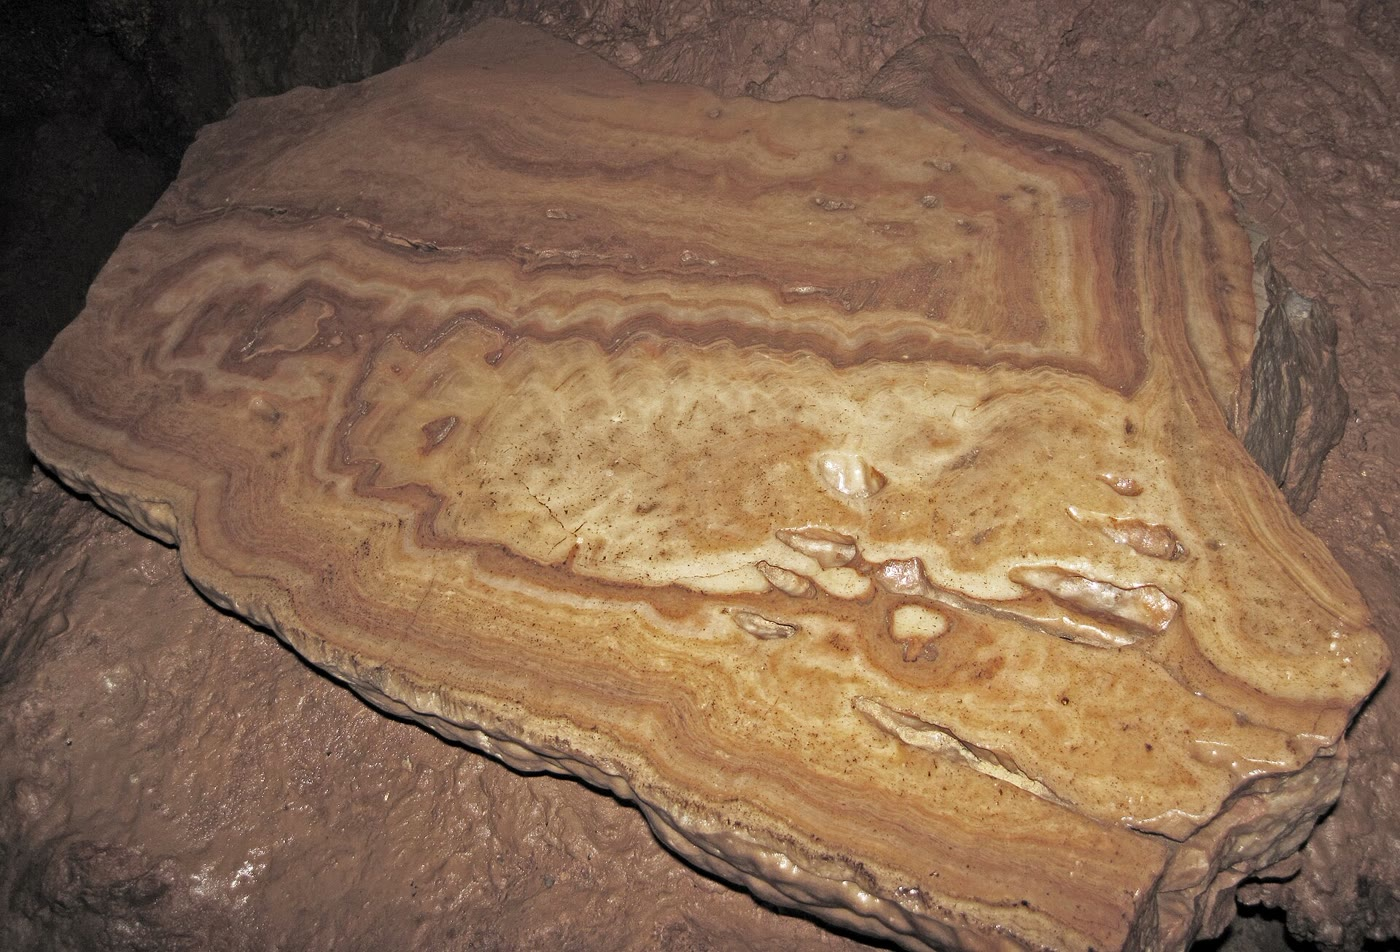
\includegraphics[width=0.62\linewidth]{images/book4/b2-24-speleothem.jpg}
\par\smallskip{\small A cut and polished section of a calcite \omterm{def:b2:climate-proxies:archives}{speleothem} from Diamond Caverns,
Kentucky, coloured by iron oxide impurities: each band was once the surface of the deposit.
(James St.~John, CC BY 2.0, via Wikimedia Commons.)}
\end{omfigure}
% ledger: photo:b2-24-speleothem

In the deep basin of Crawford Lake, in Ontario, the bottom water, saltier and more alkaline than
the water above it, holds no animals large enough to stir the mud, although it is well
oxygenated, and every year adds a couplet: a layer of organic matter, capped by the
calcite that precipitates each summer from the alkaline surface water. Lake sediments also keep
the pollen of the surrounding vegetation, read by pollen analysis; varved or not, they record
the land.
% ledger: mccarthy23:varves, mccarthy23:no-bioturbation, ncei:pollen

\section{Age models}\label{sec:b2:climate-proxies:age}

A proxy without a date is a curiosity. Every archive needs a relation between depth, or ring, or
band, and age.

\begin{definition}[Age model; annual layer counting]\label{def:b2:climate-proxies:age-model}
An \emph{age model}\index{age model} is the function that assigns an age, with its uncertainty, to
every depth of an archive. \emph{Annual layer counting}\index{annual layer counting} builds an age
model by counting, from the top down, the layers that each record one year (ice layers, \omterm{def:b2:climate-proxies:archives}{varves},
bands), each layer whose annual nature is doubtful being counted as half a year plus or minus
half a year.
\end{definition}
% ledger: svensson08:gicc05, mccarthy23:varves

\begin{method}[Building an age model]\label{met:b2:climate-proxies:age-model}
\begin{enumerate}
  \item Where the archive has annual layers, count them from a known top, recording the uncertain
        ones separately.
  \item Where it has none, or they cannot be resolved, fix \emph{tie points}: depths dated
        independently, by radiocarbon or other radiometric methods, by a dated volcanic ash, or by
        matching a well-dated record.
  \item Between tie points, interpolate, linearly in depth if nothing better is known, or with a
        model of how the archive accumulated and thinned.
  \item Carry the uncertainty of each step to every depth.
\end{enumerate}
\end{method}
% ledger: svensson08:gicc05, noaa:gisp2-layers, ncei:speleothem

The Greenland Ice Core Chronology 2005, GICC05, counts annual layers in three Greenland cores, and
in the glacial part in the NorthGRIP core alone, over the last \num{60000} years; its ages are
given in years before AD 2000, written b2k. The uncertain layers, counted as $\frac12 \pm \frac12$,
add up to the \emph{maximum counting error}, which the authors regard as two standard deviations.
At the start of the Holocene, 11\,703 years b2k, it is 50 years; at the onset of the
Greenland interstadial 17, \num{59440} years b2k, it is \num{1287} years.
% ledger: svensson08:gicc05, svensson08:table1

\begin{proposition}[Growth of a counting error]\label{prop:b2:climate-proxies:counting}
Let a count contain $n$ uncertain layers, each counted as $\frac12$ with an error of standard
deviation $\frac12$. If the errors of the layers are independent, the standard deviation of the
total is $\frac12\sqrt{n}$; if they are all of the same sign, the error of the total is
$\frac12 n$.
\end{proposition}

\begin{proof}
The variance of a sum of independent errors is the sum of their variances: $n \times
(\frac12)^2$, whose square root is $\frac12\sqrt{n}$. If every layer errs the same way, the
errors add as numbers: $n \times \frac12$.
\end{proof}

At GI-17, the \num{1287} years of maximum counting error mean \num{2574} uncertain layers. Were
their errors independent, the total would be uncertain by only $\frac12\sqrt{2574} = 25$ years.
The linear sum is the cautious choice: the doubtful layers of one stretch of ice are judged by
the same counters with the same criteria, and there is no reason to expect their errors to cancel.
The older part of the record was counted independently by two of the authors; their counts
differ by less than the absolute error, though locally by more than the final counting error. The
maximum counting error averages about \qty{1}{\percent} of the age in the Holocene and
\qty{5}{\percent} in the glacial part.
% ledger: svensson08:gicc05, svensson08:table1, svensson08:two-counters

\begin{omfigure}
\centering
% figdata/bachelor-2/proxies.py part gicc05
\begin{tikzpicture}
\begin{groupplot}[group style={group size=2 by 1, horizontal sep=1.7cm},
  tick label style={font=\scriptsize}, label style={font=\small}, height=5.4cm,
  width=0.48\linewidth, xmin=0, xmax=62, xlabel={GICC05 age (\unit{ka} b2k)}]
\nextgroupplot[ymin=1450, ymax=2450, y dir=reverse, ylabel={NorthGRIP depth (\unit{m})},
  title={a\enspace depth and age}, title style={font=\scriptsize}]
\addplot[black, mark=*, mark size=1.1pt] table[x=age_ka, y=depth_m]
  {figdata/out/bachelor-2-proxies-gicc05.dat};
\nextgroupplot[ymode=log, ymin=2, ymax=30000, ylabel={uncertainty (years)},
  title={b\enspace counting uncertainty}, title style={font=\scriptsize},
  legend style={font=\scriptsize, at={(0.03,0.97)}, anchor=north west, draw=none},
  legend cell align=left]
\addplot[ocRed, mark=*, mark size=1.1pt] table[x=age_ka, y=err_yr]
  {figdata/out/bachelor-2-proxies-gicc05.dat};
\addlegendentry{maximum counting error}
\addplot[ocBlue, mark=o, mark size=1.1pt] table[x=age_ka, y=err_random_yr]
  {figdata/out/bachelor-2-proxies-gicc05.dat};
\addlegendentry{if independent}
\end{groupplot}
\end{tikzpicture}
\par\smallskip{\small The GICC05 chronology at 18 climate events from the start of the Holocene to
\qty{59.44}{ka}: (a) depth in the NorthGRIP core against age; the curve flattens as the annual
layers thin with depth, each thousand years taking up fewer metres of ice; (b) the maximum counting error, and the error the same number of uncertain
layers would give if their errors were independent (\cref{prop:b2:climate-proxies:counting});
logarithmic scale. Data: Svensson et al.\ (2008), Table 1.}
\end{omfigure}
% ledger: svensson08:table1, svensson08:gicc05

Annual layers thin with depth, because the ice flows and spreads as it sinks: between the start of
the Holocene and GI-1, the mean layer is \qty{3.75}{cm} thick in NorthGRIP; between GI-16 and
GI-17, \qty{1.54}{cm}; around \qty{100}{ka}, flow models put it near \qty{1}{cm}. The thinner the layers, the harder
they are to tell apart.
% ledger: svensson08:table1, svensson08:gicc05

\section{Calibration}\label{sec:b2:climate-proxies:calibration}

Every number read from a proxy comes through a calibration.

\begin{definition}[Proxy calibration]\label{def:b2:climate-proxies:calibration}
A \emph{proxy calibration}\index{proxy calibration} is the empirical or theoretical relation that
converts the value of a proxy into the climate variable it stands for, established on samples for
which both are known, together with its uncertainty and the range of conditions over which it is
valid.
\end{definition}
% ledger: morley24:mgca, miller20:paleotemp

The samples for which both are known are modern: shells caught in plankton tows, the tops of sediment cores compared with the water above them, recent snow compared with the
temperature of its site, the outer rings of trees compared with the records of a weather station.
The relation is then fitted by least squares; for an exponential law such as the Mg/Ca
calibration the fit is made on the logarithm, which turns $\text{Mg/Ca} = B\,\mathrm{e}^{AT}$ into
the straight line $\ln(\text{Mg/Ca}) = \ln B + AT$. A calibration is validated on samples that
were not used to fit it: part of the modern data is put aside and predicted.
% ledger: morley24:mgca, werner18:slopes, ncei:tree-ring

Three limits remain. A calibration measured across space, from place to place today, may not hold
in time, as the Greenland ice has shown. A calibration measured over today's range of conditions
must be extrapolated with care: the Mg/Ca of shells departs from its law at low temperatures, where
another variable, the carbonate ion, takes over. And a relation that is linear over a small range
may not be linear over a large one, as the \omterm{def:b2:climate-proxies:ice-volume}{ice-volume effect} is not. The method of this chapter
answers them in the same way: measure two independent proxies on the same sample, and let each
check the other.
% ledger: werner18:slopes, morley24:mgca, rohling21:linear

\section*{Exercises}\label{sec:b2:climate-proxies:exercises}

Data for the exercises, unless stated otherwise: mean ocean depth $H = \qty{3682.2}{m}$, ocean
area \qty{361.84e6}{km^2}; the benthic calibration of \cref{prop:b2:climate-proxies:benthic}; the
planktonic calibration $\text{Mg/Ca} = 0.4\,\mathrm{e}^{0.09T}$ (\unit{mmol/mol}, \unit{\celsius});
$\delta$ values of waters and ice in per mil \omterm{def:b2:isotope-geochemistry:standards}{VSMOW}, of calcite in per mil \omterm{def:b2:isotope-geochemistry:standards}{VPDB}.
% ledger: charette:ocean-volume, miller20:paleotemp, morley24:mgca

\begin{exercise}[$\star$]\label{exo:b2:climate-proxies:1}
Today the continental ice holds about \qty{27.5e6}{km^3} and the ocean \qty{1350e6}{km^3} of
water (take the volumes as amounts of water). (a) If the ice has a mean $\delta^{18}$O of $-30$ per
mil and the ocean 0, what is the $\delta^{18}$O of the whole hydrosphere, neglecting the fresh
water? (b) If all the ice melted, what would the $\delta^{18}$O of the ocean become? (c) What
fraction of the water is ice?
\end{exercise}
% ledger: white13c9:ice-mass

\begin{exercise}[$\star$]\label{exo:b2:climate-proxies:2}
A benthic shell has $\delta^{18}\mathrm{O}_{\mathrm{b}} = 2.50$ per mil. (a) Compute its
temperature if the sea water had $\delta^{18}\mathrm{O}_{\mathrm{sw}} = 0$. (b) Compute it if the
sea water had $+1.0$ per mil. (c) Another shell, from the same water at $0$ per mil, has
$2.71$ per mil: by how much was its water colder?
\end{exercise}
% ledger: miller20:paleotemp

\begin{exercise}[$\star$]\label{exo:b2:climate-proxies:3}
(a) Compute the Mg/Ca ratio of the planktonic calibration at \qty{10}{\celsius} and at
\qty{20}{\celsius}. (b) By what factor does the ratio grow over these ten degrees, and by what
percentage per degree? (c) Compute the temperature of shells with Mg/Ca = 2.0 and
\qty{1.0}{mmol/mol}.
\end{exercise}
% ledger: morley24:mgca

\begin{exercise}[$\star$]\label{exo:b2:climate-proxies:4}
A chronology of subfossil yews runs from 2668 to 2213 BCE. (a) How many years does it cover,
counting both end years? (b) Why does a chronology built from many trees deserve more trust than
the count of the rings of a single tree? (c) Why would you expect \omterm{def:b2:climate-proxies:dendro}{cross-dating} to be easier for
trees near the cold tree line than for trees in a mild, moist lowland forest?
\end{exercise}
% ledger: bebchuk26:crossdating

\begin{exercise}[$\star\star$]\label{exo:b2:climate-proxies:5}
(a) With \cref{prop:b2:climate-proxies:mass-balance}, compute the \omterm{def:b2:climate-proxies:ice-volume}{ice-volume effect} for a sea-level
fall of \qty{125}{m} and of \qty{134}{m}, with ice at $-40$ per mil. (b) Compute it for
\qty{130}{m} with ice at $-30$, $-35$ and $-50$ per mil. (c) Which mean composition of the ice
would make the effect of a \qty{130}{m} fall equal to the \num{1.0} per mil measured in pore
waters? Compare with the compositions of the present ice sheets.
\end{exercise}
% ledger: ipcc:lgm-sea, white:d18o, miller20:ice-cal, wharton26:deep

\begin{exercise}[$\star\star$]\label{exo:b2:climate-proxies:6}
Compare the two calibrations of the Mg/Ca of the same planktonic species: the one predicted from
temperature alone, $0.4\,\mathrm{e}^{0.09T}$, and the fit $0.372\,\mathrm{e}^{0.0936T}$. (a) At
what temperature do they agree? (b) At \qty{2}{\celsius}, by what percentage is the fitted ratio
lower than the predicted one? (c) A shell grown at \qty{2}{\celsius} follows the fitted law; what
temperature would the predicted law give for it?
\end{exercise}
% ledger: morley24:mgca

\begin{exercise}[$\star\star$]\label{exo:b2:climate-proxies:7}
In the NorthGRIP core, the start of the Holocene lies at \qty{1492.45}{m} and \num{11703} years
b2k, the onset of GI-1 at \qty{1604.64}{m} and \num{14692} years; the onset of GI-16 at
\qty{2402.55}{m} and \num{58280} years, that of GI-17 at \qty{2420.44}{m} and \num{59440} years.
(a) Compute the mean thickness of the annual layers in each interval. (b) Why are they thinner
deeper down? (c) Why does \omterm{def:b2:climate-proxies:age-model}{annual layer counting} become impossible at some depth?
\end{exercise}
% ledger: svensson08:table1, svensson08:gicc05

\begin{exercise}[$\star\star$]\label{exo:b2:climate-proxies:8}
Use the first two tie points of \cref{exo:b2:climate-proxies:7}, with maximum counting errors of 50
and 93 years. (a) By linear interpolation in depth, give the age of the ice at \qty{1550}{m}.
(b) Express it in years before 1950. (c) Interpolate the uncertainty in the same way.
\end{exercise}
% ledger: svensson08:table1

\begin{exercise}[$\star\star$]\label{exo:b2:climate-proxies:9}
The maximum counting error of GICC05 is 93 years at GI-1 and \num{1287} years at GI-17. (a) How many
uncertain layers does each represent? (b) What would the uncertainty be if the errors of these
layers were independent, each of standard deviation half a year? (c) By what factor does the
linear sum exceed the independent estimate in each case, and why does the factor grow with depth?
\end{exercise}
% ledger: svensson08:gicc05, svensson08:table1

\begin{exercise}[$\star\star\star$]\label{exo:b2:climate-proxies:10}
At EPICA Dome C the mean $\delta$D of the ice is $-396.6$ per mil over the last two thousand years
and $-441.7$ per mil over 19 to \qty{23}{ka}. (a) The Antarctic spatial slope of $\delta^{18}$O is
\num{0.8} per mil per degree. With the \omterm{prop:b2:isotope-geochemistry:mwl}{meteoric water line}, convert it to a slope of $\delta$D and
estimate the glacial cooling. (b) The glacial ocean was \num{1.0} per mil heavier in
$\delta^{18}$O, so the snow formed from it was heavier too. Assuming the $\delta$D of the ocean
changed eight times as much, correct the glacial $\delta$D and estimate the cooling again.
(c) The published anomaly is $-0.09$ and \qty{-9.39}{\celsius} for the two periods; what slope of
$\delta$D per degree does that imply, and what other correction does the published series contain?
\end{exercise}
% ledger: data:b4-proxies, werner18:slopes, kc98:mwl, wharton26:deep, jouzel07:edc-corr

\begin{exercise}[$\star\star\star$]\label{exo:b2:climate-proxies:11}
A calibration of the Mg/Ca of a planktonic species uses six core-top samples (water temperature,
Mg/Ca in \unit{mmol/mol}): (4, 0.59), (8, 0.80), (12, 1.21), (16, 1.65), (20, 2.47), (24, 3.41).
(a) Fit $\ln(\text{Mg/Ca}) = \ln B + AT$ by least squares, and give $A$ and $B$. (b) Compute the
residuals of the logarithm, and compare the fit with the law $0.4\,\mathrm{e}^{0.09T}$. (c) Give the
temperature of a glacial shell with Mg/Ca = 1.30. (d) A shell has Mg/Ca = 0.45: compute its
temperature, and say why this value deserves less trust than the previous one.
\end{exercise}
% ledger: morley24:mgca

\begin{exercise}[$\star\star\star$]\label{exo:b2:climate-proxies:12}
An ice sheet grows in two stages: first \qty{60}{m} of sea level is stored as ice at $-30$ per mil,
then \qty{70}{m} more as ice at $-45$ per mil. (a) Show that the mass balance of
\cref{prop:b2:climate-proxies:mass-balance} becomes $(H - h)\,\Delta\delta = -\sum_i h_i\delta_i$
for several stores of ice, and compute the \omterm{def:b2:climate-proxies:ice-volume}{ice-volume effect} after each stage. (b) What is the mean
composition of the ice at the end? (c) A linear rule, calibrated on the end state, converts
$\Delta\delta$ into sea level. What sea-level fall would it infer for the first stage, and why does
it err?
\end{exercise}
% ledger: rohling21:linear, white:d18o, miller20:ice-cal

\begin{problem}[{Weekend problem --- One shell, two signals}]\label{pb:b2:climate-proxies:1}
How much colder was the deep ocean at the Last Glacial Maximum? The $\delta^{18}$O of benthic shells
mixes the answer with the volume of the ice; this problem separates the two. Use the data of the
exercises; sea level stood 125 to \qty{134}{m} below today's, and the ice of the North American ice
sheet is thought to have had a $\delta^{18}$O of about $-40$ per mil.

\medskip\noindent\textbf{Part I --- The ice on land.}
\begin{enumerate}
  \item Compute the volume of water removed from the ocean by a sea-level fall of \qty{130}{m}.
  \item Compute the \omterm{def:b2:climate-proxies:ice-volume}{ice-volume effect} of that fall with ice at $-40$ per mil.
  \item Compute it for falls of \qty{125}{m} and \qty{134}{m}.
  \item Compute it for \qty{130}{m} with ice at $-35$ and at $-50$ per mil. Which uncertainty
        matters more, that of the sea level or that of the ice?
  \item The pore waters of glacial sediments give $1.0 \pm 0.1$ per mil. What mean composition
        of the ice would a fall of \qty{130}{m} require to produce it?
  \item Compute the shift per metre of sea level for small falls with ice at $-40$ per mil, and
        compare with the value of \num{0.011} per mil per metre derived from dated sea levels.
\end{enumerate}

\medskip\noindent\textbf{Part II --- Two thermometers.}
\begin{enumerate}[resume]
  \item Show from \cref{prop:b2:climate-proxies:benthic} that a cooling of \qty{1}{\celsius} at
        constant water composition raises $\delta^{18}\mathrm{O}_{\mathrm{b}}$ by \num{0.21} per mil.
  \item Compute $\delta^{18}\mathrm{O}_{\mathrm{b}}$ of a benthic shell grown today in water at
        \qty{2.0}{\celsius} with $\delta^{18}\mathrm{O}_{\mathrm{sw}} = 0$.
  \item Compute it for a glacial shell grown in water at \qty{-1.0}{\celsius} with
        $\delta^{18}\mathrm{O}_{\mathrm{sw}} = +1.0$ per mil. What is the change between the two
        shells, and how much of it is due to the water's composition?
  \item A planktonic shell has Mg/Ca = \qty{2.0}{mmol/mol}. Compute its temperature.
  \item Low-magnesium benthic shells gain about \qty{0.1}{mmol/mol} per degree. A glacial shell has
        a Mg/Ca \qty{0.18}{mmol/mol} lower than a modern one of the same species from the same
        place. What cooling does that indicate?
  \item Why does Mg/Ca give a temperature that does not depend on the volume of ice?
\end{enumerate}

\medskip\noindent\textbf{Part III --- The residual.}
The LR04 stack reads \num{3.23} per mil today and \num{4.92} per mil on average over 19 to
\qty{23}{ka}.
\begin{enumerate}[resume]
  \item Compute the change of the stack between today and the Last Glacial Maximum.
  \item If all of it were \omterm{def:b2:climate-proxies:ice-volume}{ice-volume effect}, with ice at $-40$ per mil, what sea-level fall would it
        imply (invert \cref{prop:b2:climate-proxies:mass-balance})? Is that consistent with the
        sea-level evidence?
  \item Take the \omterm{def:b2:climate-proxies:ice-volume}{ice-volume effect} of question 2. What residual remains for the temperature, and
        what cooling of the deep water does it give?
  \item Take instead the pore-water value, \num{1.0} per mil. What residual and what cooling?
  \item Another reconstruction uses \num{0.25} per mil per degree. Repeat the two estimates with it.
  \item Today the North Atlantic Deep Water is at 2 to \qty{4}{\celsius} and the Antarctic Bottom
        Water at 0 to \qty{1}{\celsius}; pore waters put them at $-1.1$ and \qty{-1.9}{\celsius}
        in the glacial ocean, and the Mg/Ca of benthic shells finds the deep North-West Atlantic
        only about \qty{1.8}{\celsius} colder. What range of cooling do these give, and which of the
        two estimates of questions 15 and 16 do they favour?
\end{enumerate}

\medskip\noindent\textbf{Part IV --- The view from the ice.}
At EPICA Dome C the mean $\delta$D is $-396.6$ per mil over the last two thousand years and
$-441.7$ per mil over 19 to \qty{23}{ka}; the published temperature anomaly is $-0.09$ and
\qty{-9.39}{\celsius}.
\begin{enumerate}[resume]
  \item Compute the change of $\delta$D.
  \item With a $\delta^{18}$O slope of \num{0.8} per mil per degree and the \omterm{prop:b2:isotope-geochemistry:mwl}{meteoric water line},
        estimate the cooling at Dome C.
  \item Compute the published cooling, and the slope of $\delta$D per degree it implies.
  \item The global mean surface was 5 to \qty{7}{\celsius} colder at the Last Glacial Maximum.
        Rank the coolings of Dome C, of the globe and of the deep ocean.
  \item Why can the deep ocean not have cooled by as much as the surface of Antarctica?
  \item To sum up: with the pore-water correction for ice volume, by how much was the deep ocean
        colder at the Last Glacial Maximum than today?
\end{enumerate}
\end{problem}
% ledger: charette:ocean-volume, ipcc:lgm-sea, miller20:ice-cal, white:d18o, white13c9:ice-volume, wharton26:deep, miller20:paleotemp, morley24:mgca, data:b4-proxies, rohling21:linear, werner18:slopes, kc98:mwl, ipcc:lgm-cooling
